\section{Further invstigation of the Second Run~\label{sec:u_s_time_hist}} 
This section exhibits user and system time histograms on the second run of 
INC with its task length increasing from 1 second to 4096 seconds, via SEDONA. 
The detailed description of the base data is from Table~\ref{tab:exp_notes2}.

\subsection{User Time}

\begin{figure}[hp!]
	\centering
	\subfigure[User time frequency on INC1]{
		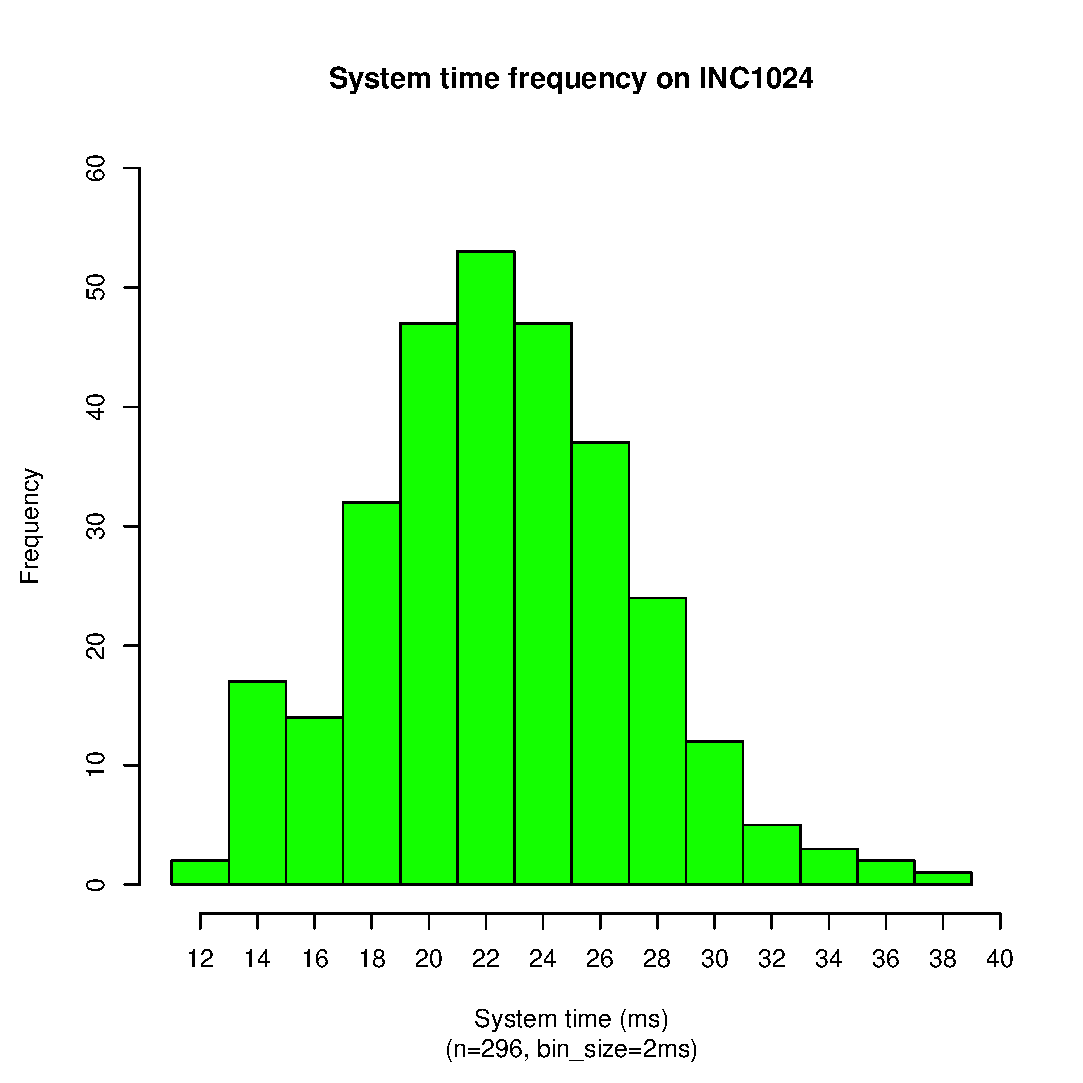
\includegraphics[scale=0.43]{u_s_time/1_sec_ut_hist.eps}
		\label{fig:inc1_ut_hist}
	}
	\subfigure[User time frequency on INC2]{
		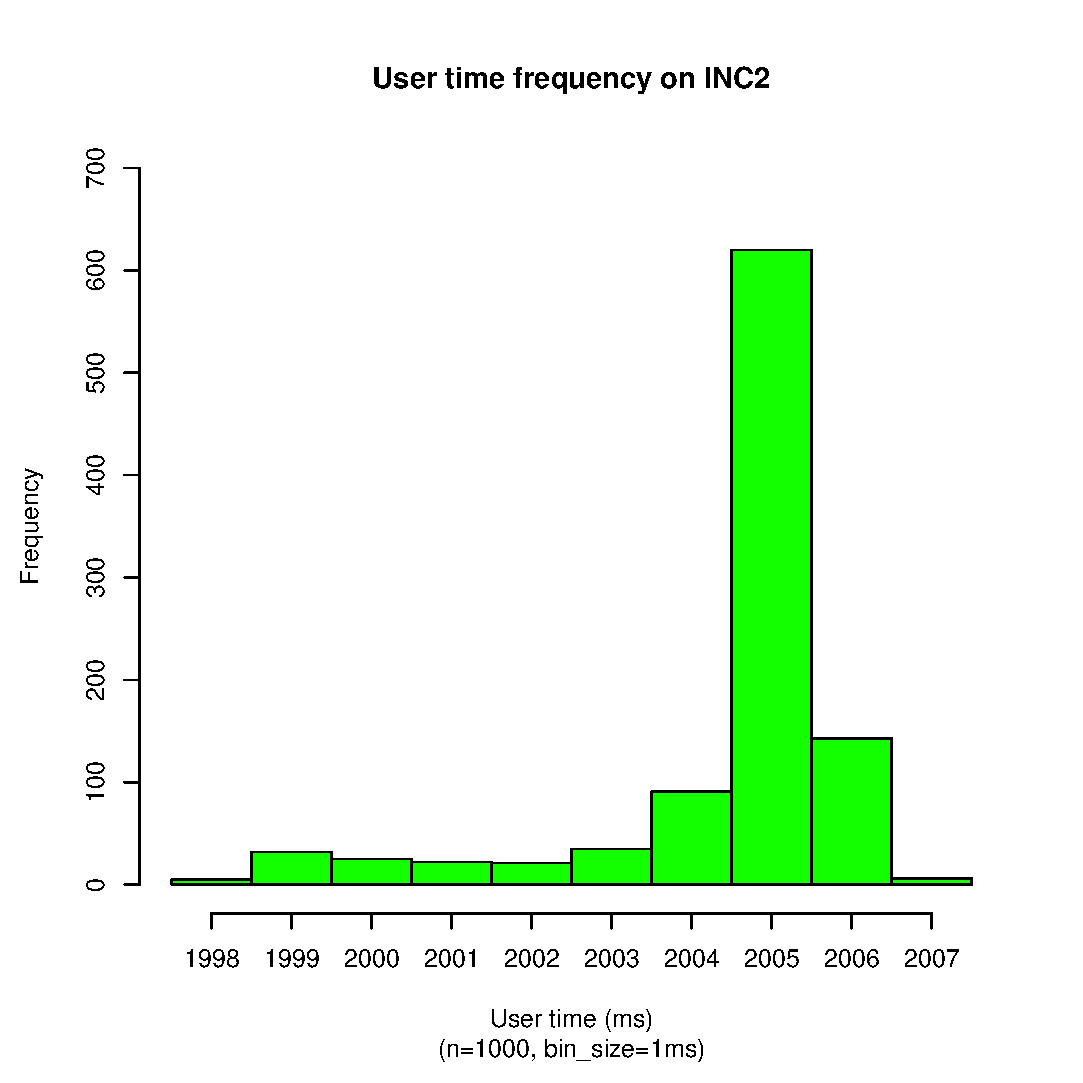
\includegraphics[scale=0.43]{u_s_time/2_sec_ut_hist.eps}
		\label{fig:inc2_ut_hist}
	}
	\subfigure[User time frequency on INC4]{
		\includegraphics[scale=0.43]{u_s_time/4_sec_ut_hist.eps}
		\label{fig:inc4_ut_hist}
	}
	\subfigure[User time frequency on INC8]{
		\includegraphics[scale=0.43]{u_s_time/8_sec_ut_hist.eps}
		\label{fig:inc8_ut_hist}
	}
	\caption{User Time Histograms of INC1 ... INC8~\label{fig:ut_hist1}}
\end{figure}

\begin{figure}[hp!]
	\centering
	\subfigure[User time frequency on INC16]{
		\includegraphics[scale=0.43]{u_s_time/16_sec_ut_hist.eps}
		\label{fig:inc16_ut_hist}
	}
	\subfigure[User time frequency on INC32]{
		\includegraphics[scale=0.43]{u_s_time/32_sec_ut_hist.eps}
		\label{fig:inc32_ut_hist}
	}
	\subfigure[User time frequency on INC64]{
		\includegraphics[scale=0.43]{u_s_time/64_sec_ut_hist.eps}
		\label{fig:inc64_ut_hist}
	}
	\caption{User Time Histograms of INC16 ... INC64~\label{fig:ut_hist2}}
\end{figure}

\begin{figure}[hp!]
	\centering
	\subfigure[User time frequency on INC128]{
		\includegraphics[scale=0.43]{u_s_time/128_sec_ut_hist.eps}
		\label{fig:inc128_ut_hist}
	}
	\subfigure[User time frequency on INC256]{
		\includegraphics[scale=0.43]{u_s_time/256_sec_ut_hist.eps}
		\label{fig:inc256_ut_hist}
	}
	\subfigure[User time frequency on INC512]{
		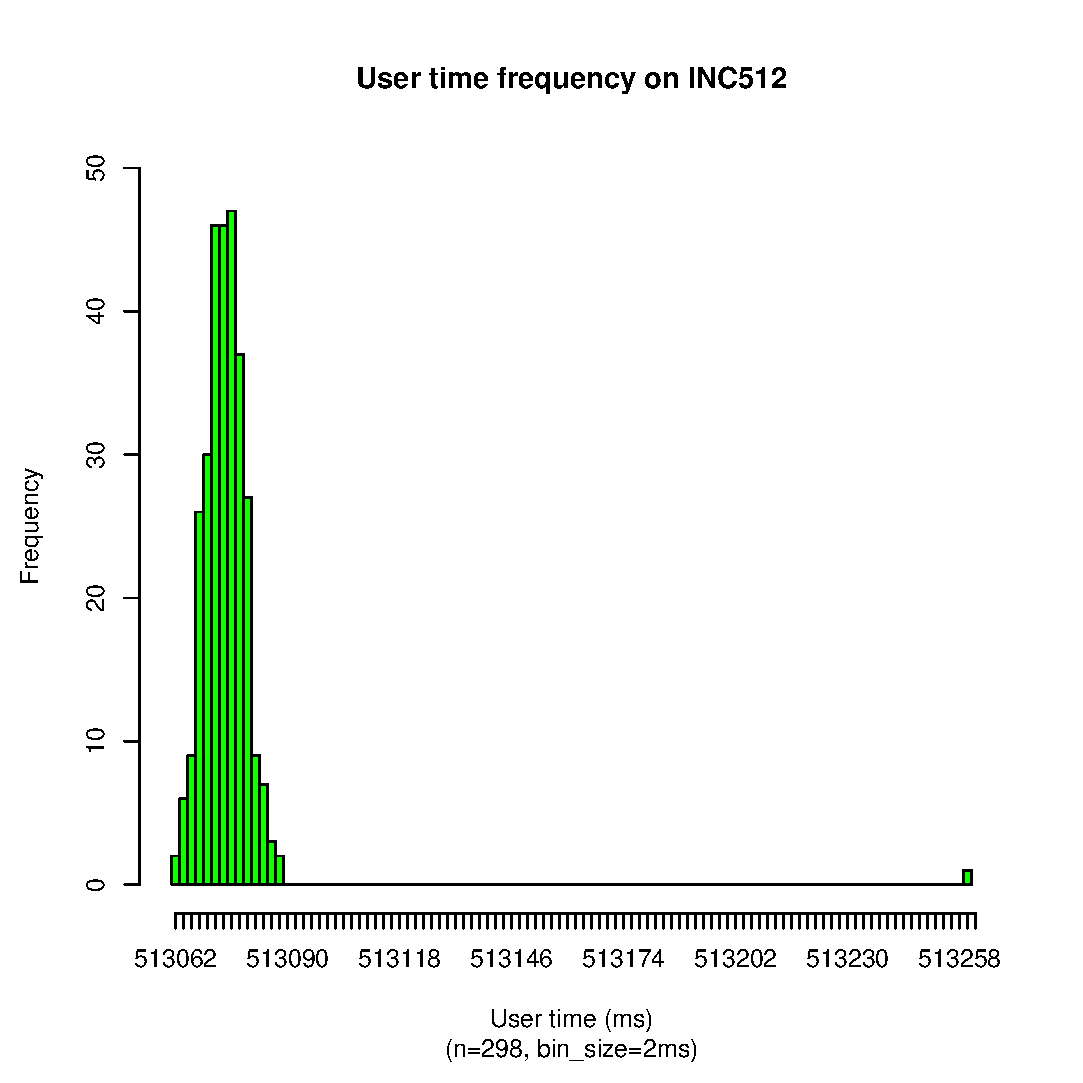
\includegraphics[scale=0.43]{u_s_time/512_sec_ut_hist.eps}
		\label{fig:inc512_ut_hist}
	}
	\subfigure[User time frequency on INC1024]{
		\includegraphics[scale=0.43]{u_s_time/1024_sec_ut_hist.eps}
		\label{fig:inc1024_ut_hist}
	}
	\caption{User Time Histograms of INC128 ... INC1024~\label{fig:ut_hist3}}
\end{figure}

\begin{figure}[hp!]
	\centering
	\subfigure[User time frequency on INC2048]{
		\includegraphics[scale=0.43]{u_s_time/2048_sec_ut_hist.eps}
		\label{fig:inc2048_ut_hist}
	}
	\subfigure[User time frequency on INC4096]{
		\includegraphics[scale=0.43]{u_s_time/4096_sec_ut_hist.eps}
		\label{fig:inc4096_ut_hist}
	}
	\caption{User Time Histograms of INC2048 and INC4096~\label{fig:ut_hist4}}
\end{figure}

\vspace\fill
\clearpage

\subsection{System Time}

\begin{figure}[hp!]
	\centering
	\subfigure[System time frequency on INC1]{
		\includegraphics[scale=0.43]{u_s_time/1_sec_st_hist.eps}
		\label{fig:inc1_hist_v5}
	}
	\subfigure[System time frequency on INC2]{
		\includegraphics[scale=0.43]{u_s_time/2_sec_st_hist.eps}
		\label{fig:inc2_hist_st}
	}
	\subfigure[System time frequency on INC4]{
		\includegraphics[scale=0.43]{u_s_time/4_sec_st_hist.eps}
		\label{fig:inc4_hist_st}
	}
	\subfigure[System time frequency on INC8]{
		\includegraphics[scale=0.43]{u_s_time/8_sec_st_hist.eps}
		\label{fig:inc8_hist_st}
	}
	\caption{System Time Histograms of INC1 ... INC8~\label{fig:st_hist1}}
\end{figure}

\begin{figure}[hp!]
	\centering
	\subfigure[System time frequency on INC16]{
		\includegraphics[scale=0.43]{u_s_time/16_sec_st_hist.eps}
		\label{fig:inc16_hist_st}
	}
	\subfigure[System time frequency on INC32]{
		\includegraphics[scale=0.43]{u_s_time/32_sec_st_hist.eps}
		\label{fig:inc32_hist_st}
	}
	\subfigure[System time frequency on INC64]{
		\includegraphics[scale=0.43]{u_s_time/64_sec_st_hist.eps}
		\label{fig:inc64_hist_st}
	}
	\caption{System Time Histograms of INC16 ... INC64\label{fig:st_hist2}}
\end{figure}

\begin{figure}[hp!]
	\centering
	\subfigure[System time frequency on INC128]{
		\includegraphics[scale=0.43]{u_s_time/128_sec_st_hist.eps}
		\label{fig:inc128_hist_st}
	}
	\subfigure[System time frequency on INC256]{
		\includegraphics[scale=0.43]{u_s_time/256_sec_st_hist.eps}
		\label{fig:inc256_hist_st}
	}
	\subfigure[System time frequency on INC512]{
		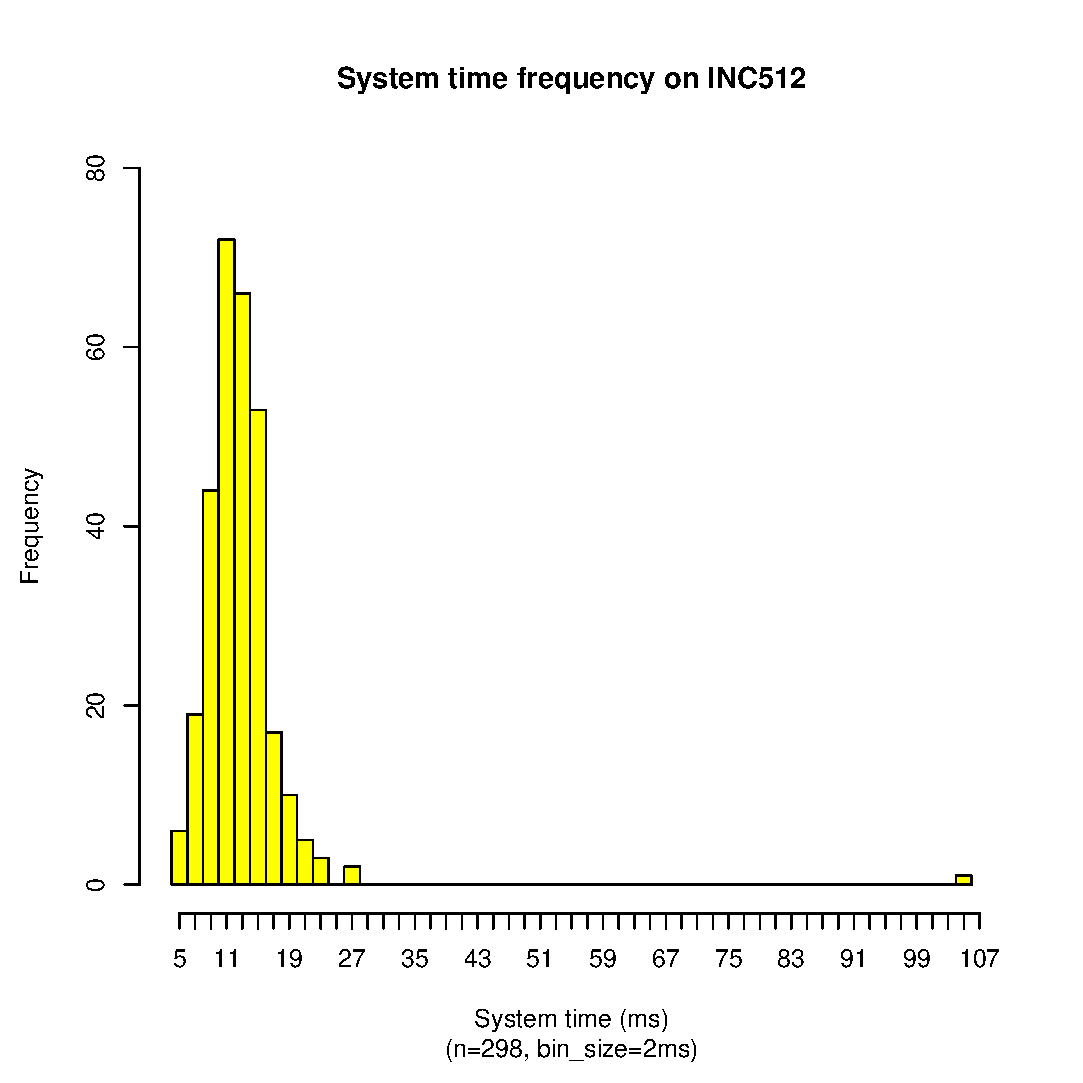
\includegraphics[scale=0.43]{u_s_time/512_sec_st_hist.eps}
		\label{fig:inc512_hist_st}
	}
	\subfigure[System time frequency on INC1024]{
		\includegraphics[scale=0.43]{u_s_time/1024_sec_st_hist.eps}
		\label{fig:inc1024_hist_st}
	}
	\caption{System Time Histograms of INC256 ... INC1024~\label{fig:st_hist3}}
\end{figure}

\begin{figure}[t]
	\centering
	\subfigure[System time frequency on INC2048]{
		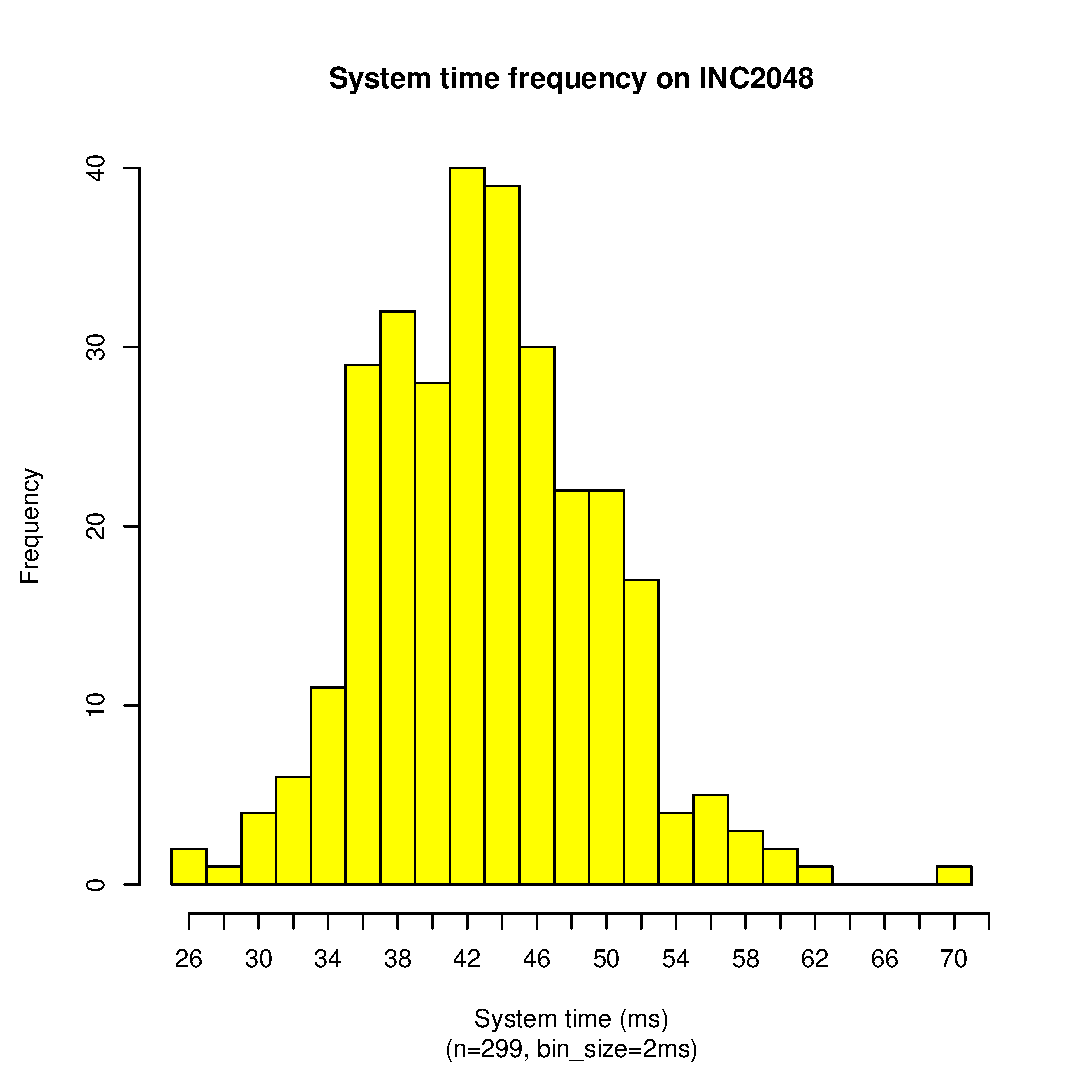
\includegraphics[scale=0.43]{u_s_time/2048_sec_st_hist.eps}
		\label{fig:inc2048_hist_st}
	}
	\subfigure[System time frequency on INC4096]{
		\includegraphics[scale=0.43]{u_s_time/4096_sec_st_hist.eps}
		\label{fig:inc4096_hist_st}
	}
	\caption{System Time Histograms of INC2048 and INC4096~\label{fig:st_hist4}}
\end{figure}

\clearpage
\pagebreak

\subsection{Correlation}

%% done
\begin{table}[h]
\begin{center}
\begin{tabular}{|c|c|c|} \hline
%Machine & Task Length (sec) & Description & Experiment Period & Relevant \linebreak Histograms\\ \hline
%{\tt sodb9} &  INC1$\sim$INC64 & 1000 samples, each & 2017-03-02 $\sim$ 2017-03-04 & Figs.~\ref{fig:s9_r1_et_hist1},~\ref{fig:s9_r1_et_hist2},~\ref{fig:s9_r1_pt_hist1}, and~\ref{fig:s9_r1_pt_hist2}\\ \hline
%{\tt sodb9} &  INC128$\sim$INC1024 & 300 samples, each & 2017-03-04 $\sim$ 2017-03-11 & 
%Figs.~\ref{fig:s9_r1_et_hist3} and~\ref{fig:s9_r1_pt_hist3}\\ \hline
%{\tt sodb10} & INC2048 & 300 samples & 2017-03-02 $\sim$ 2017-03-09 & Figs.~\ref{fig:inc2048_r1_et_hist_v5} and~\ref{fig:inc2048_r1_hist_v5}\\ \hline
%{\tt sodb12} & INC4096 & 300 samples & 2017-02-13 $\sim$ 2017-02-27 & Figs.~\ref{fig:inc4096_r1_et_hist_v5} and~\ref{fig:inc4096_r1_hist_v5}\\ \hline
 						& w/ u time & w/ s time\\ \hline
daemon u time & 0.1 & {\bf 0.3} \\ \hline
daemon s time & -0.09 & {\bf 0.19} \\ \hline
daemon minor faults & {\bf 0.11} & {\bf 0.32} \\ \hline
%read bytes & N/A & N/A
daemon read char & 0.1 & {\bf 0.32} \\ \hline
daemon read sys calls & 0.11 & {\bf 0.32} \\ \hline
daemon write bytes & 0 & {\bf 0.26} \\ \hline
daemon write char & 0.11 & {\bf 0.32}\\ \hline
%read sys calls & N/A & N/A
\end{tabular}
\end{center}
\vspace{-.2in}
\caption{Correlation of user and system time of INC4096 with some daemon measures\label{tab:corr_table}}
\end{table}

\clearpage
\newpage

\subsection{Scatter Plots on Some Significant Correlations}
The following scatter plots correspond to the correlations bold in Table~\ref{tab:corr_table}.

\begin{figure}[htp!]
	\centering
	\subfigure[User time vs. All daemon system time]{
		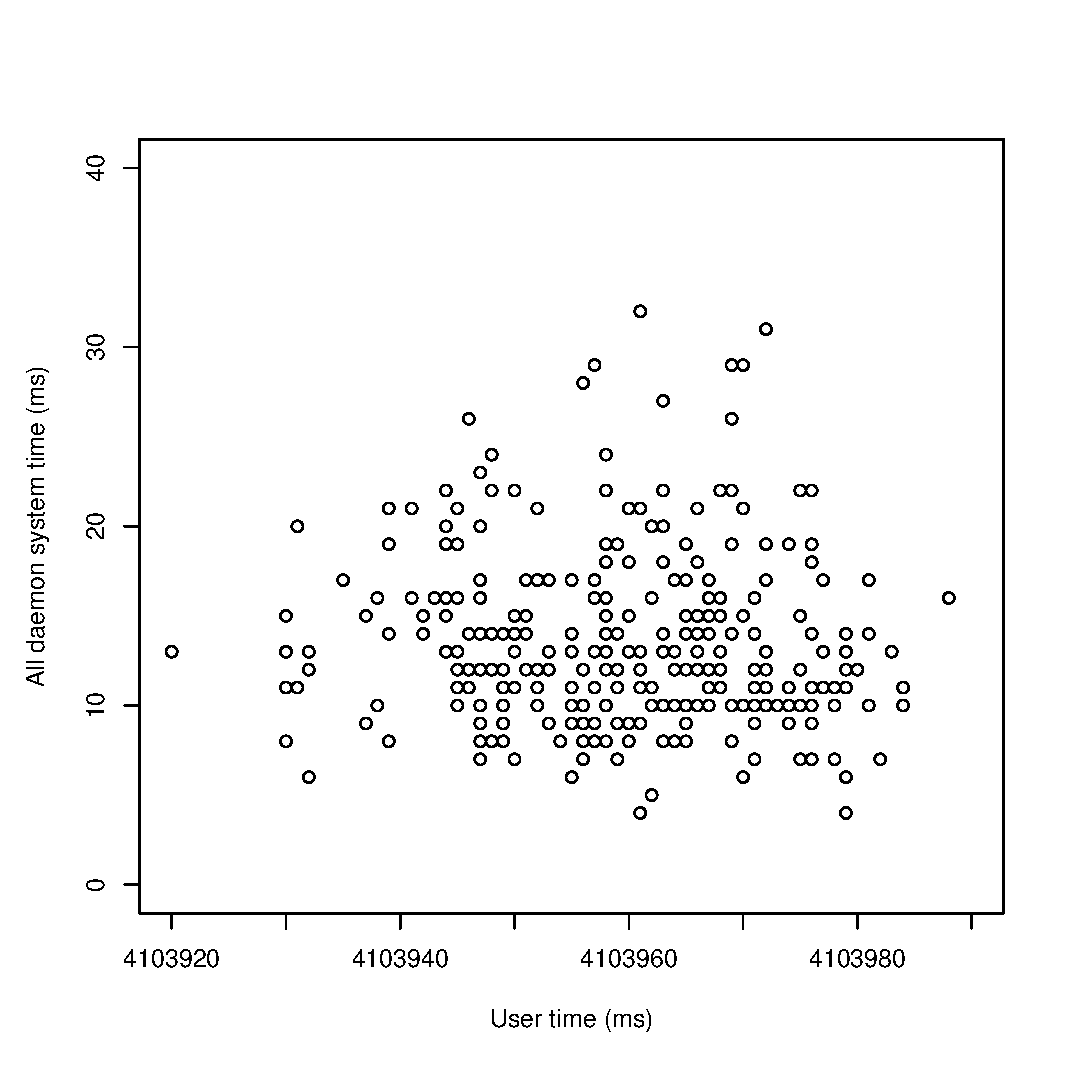
\includegraphics[scale=0.43]{u_s_time/corr_u_as_time.eps}
		\label{fig:corr_u_as_time}
	}
	\subfigure[System time vs. All daemon system time]{
		\includegraphics[scale=0.43]{u_s_time/corr_s_as_time.eps}
		\label{fig:corr_s_as_time}
	}
	\subfigure[User time vs. All daemon minor faults]{
		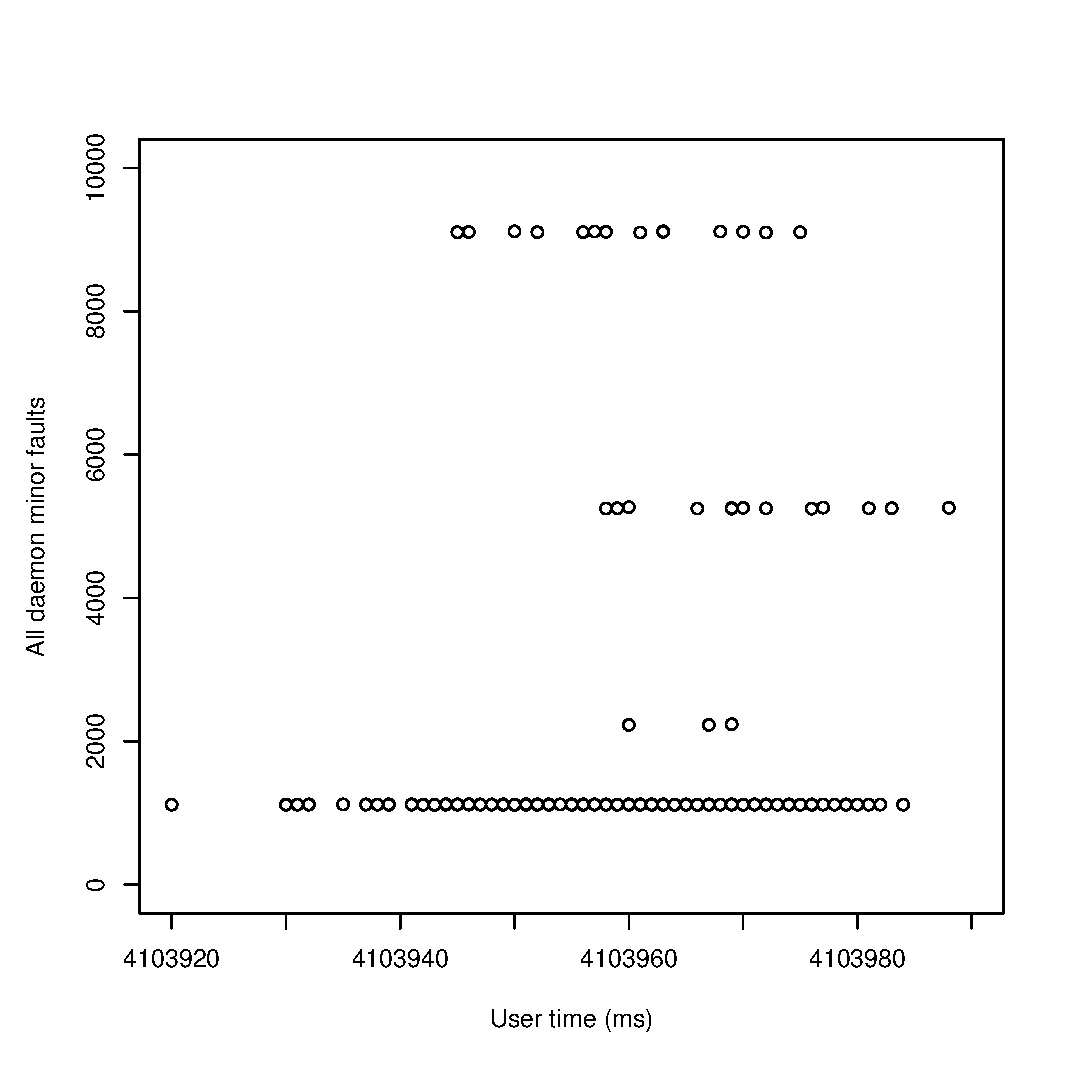
\includegraphics[scale=0.43]{u_s_time/corr_mnf_u_time.eps}
		\label{fig:corr_u_mnf}
	}
	\subfigure[System time vs. All daemon minor faults]{
		\includegraphics[scale=0.43]{u_s_time/corr_mnf_s_time.eps}
		\label{fig:corr_s_mnf}
	}
	\caption{Scatter plots between measures on INC4096~\label{fig:corr1}}
\end{figure}

\begin{figure}[htp!]
	\centering
	\subfigure[System time vs. All daemon read char]{
		\includegraphics[scale=0.43]{u_s_time/corr_s_rchar.eps}
		\label{fig:corr_s_rchar}
	}
	\subfigure[System time vs. All daemon read syscalls]{
		\includegraphics[scale=0.43]{u_s_time/corr_s_rsysc.eps}
		\label{fig:corr_s_rsysc}
	}
	\subfigure[System time vs. All daemon write bytes]{
		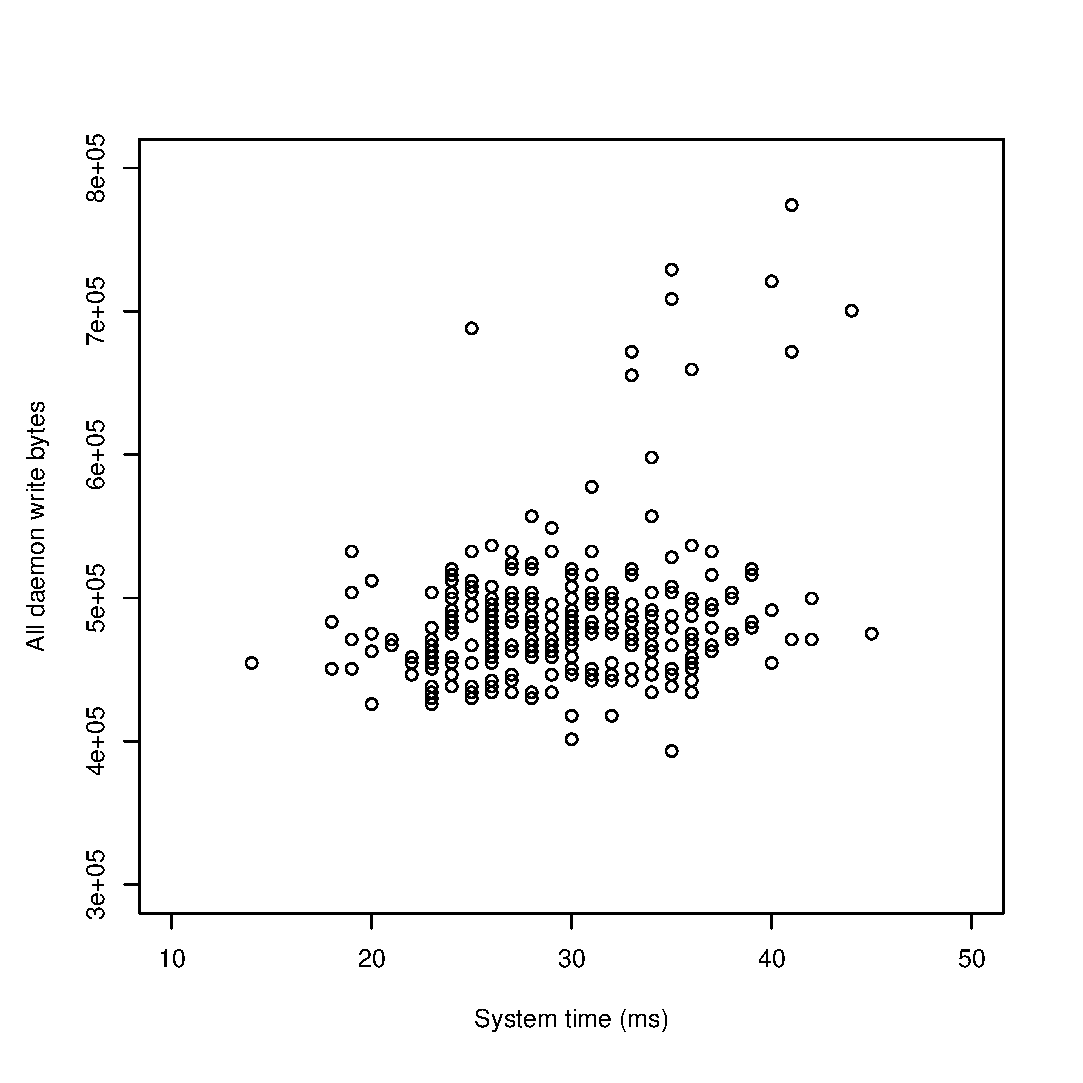
\includegraphics[scale=0.43]{u_s_time/corr_s_wbytes.eps}
		\label{fig:corr_s_wbytes}
	}
	\subfigure[System time vs. All daemon write char]{
		\includegraphics[scale=0.43]{u_s_time/corr_s_wchar.eps}
		\label{fig:corr_s_wchar}
	}
	\caption{Scatter plots between measures on INC4096~\label{fig:corr2}}
\end{figure}
